%to do
\section{background}
\label{sec:background}
\begin{comment}
\subsection{Cloud Computing}
\begin{figure}
\centering
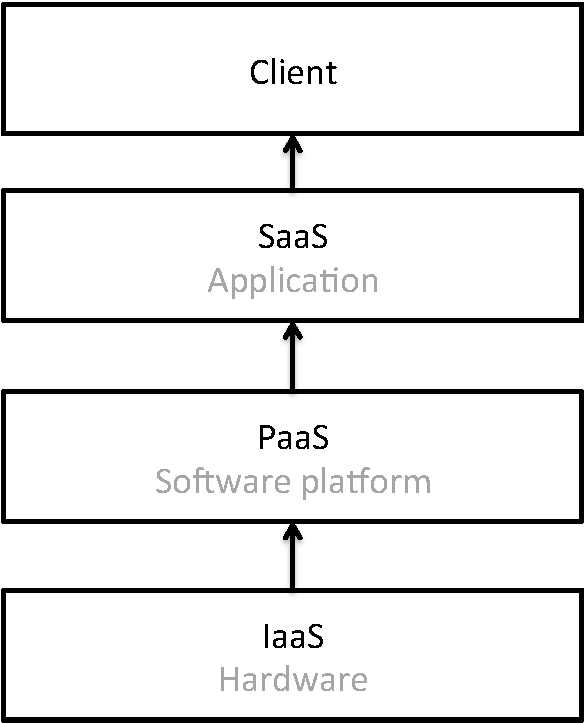
\includegraphics[width=4cm]{img/cloud_models.pdf}
\caption{the relationship of different cloud models}
\label{background:cloud models}
\end{figure}

Cloud computing refers to a model that cloud vendors provide user IT resources and charge them for
the resources they used.
Cloud vendors can offer hardware resources including CPU, memory, hard disk, network and software
resources OS, software suits and applications.
Cloud computing majorly can be classified into following three kinds of models:
\begin{enumerate}
  \item Infrastructure as a service (IaaS): cloud vendors provide only raw machines(physical or
  virtual machine), user need to set up the whole software environment including OS.
  \item Platform as a service (PaaS): in this model, cloud vendors provide hardware as well as
  software platform. Users can use it as a common computer and run applications on the platform.
  Amazon EC2 provides PaaS.
  \item Software as a service (SaaS): Cloud vendors provide a certain applications. Users don't need
  to configure the software themselves.
\end{enumerate}
The relationship of different cloud models can be shown as Figure~.\ref{background:cloud models}

Cloud computing can have following benefits:
\begin{itemize}
  \item Users don't need to care about the machine placement and maintenance.
  \item Users don't need a large number of machines to meet a temporally request peek and idle for
  the other time, Since cloud instances can set up in a few minutes when the request peek occurs.
  \item Users don't need to pay for expensive hardware and software, they just need to pay for what
  they used.
\end{itemize}
\end{comment}
\subsection{Interconnection Network vs. Shared Storage}

\begin{figure}
\centering
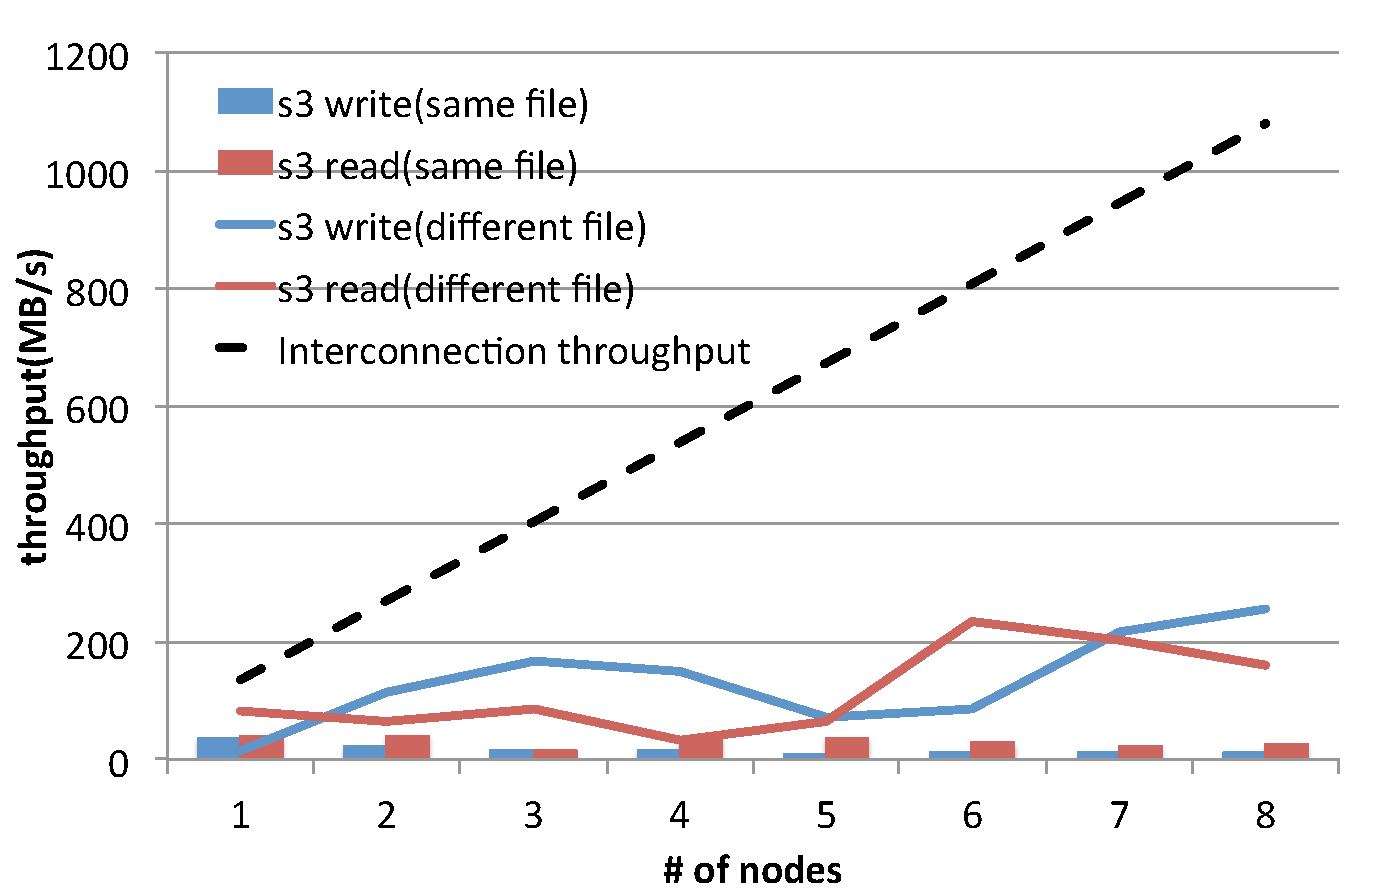
\includegraphics[width=8cm]{img/amazon_throughput}
\caption{Amazon Interconnection Network Throughput vs. Amazon S3 Throughput}
\label{background:amazon throughput}
\end{figure}

Many previous research measured the I/O throughput in cloud \cite{Chiba,Transactions_a_la_carte,
Interactive_Use_of_Cloud_Services,Amazon_S3_for_Science_Grids,anevaluation}, the I/O bandwidth of
Amazon S3 is much lower than that in HPC system, and the value is quite unstable\cite{anevaluation}.
Because the Amazon S3 data center is geographically-distributed, and connect via Internet, compare
to modern parallel file systems Amazon S3 cannot achieve a high throughput.
 
However, when we look at interconnection network throughput inside Amazon EC2,
Figure.~\ref{background:amazon throughput} shows a comparison of Amazon Interconnection Network
throughput and Amazon S3 throughput, although we only show the result up to 8 pairs of nodes, each
node achieved only 135MB/s (1GBit/s), the influence between nodes is extremely small, figure shows a perfect linear line also a strong scalability.
We measure the interconnection network by using Iperf\cite{iperf}, which was developed by NLANR/DAST
as a modern alternative for measuring TCP and UDP bandwidth performance.
When we running the
benchmark, many other users were also running applications on Amazon, so we can assume that highest
throughput 1GB/s (8Gbit/s) shown in Figure.~\ref{background:amazon throughput} is not the
maximum bandwidth of interconnection network in Amazon EC2.
As Figure.~\ref{background:amazon throughput} shows, Interconnection Network throughput inside
Amazon EC2 is proportional to numbers of nodes used, on the contrary, Amazon S3 throughput is much
lower than it, and unstable.
Also we can find that all nodes access to the same file is slower than access to different file,
it is because Amazon S3 will distribute different file over machines to increase I/O throughput,
access to the same file will be limited by S3 server machine bandwidth, and will cause connection
conflict.
Our proposal system takes advantage of the characteristic of
Interconnection network inside cloud system to burst I/O throughput.

\subsection{Burst Buffer}
\begin{figure}
\centering
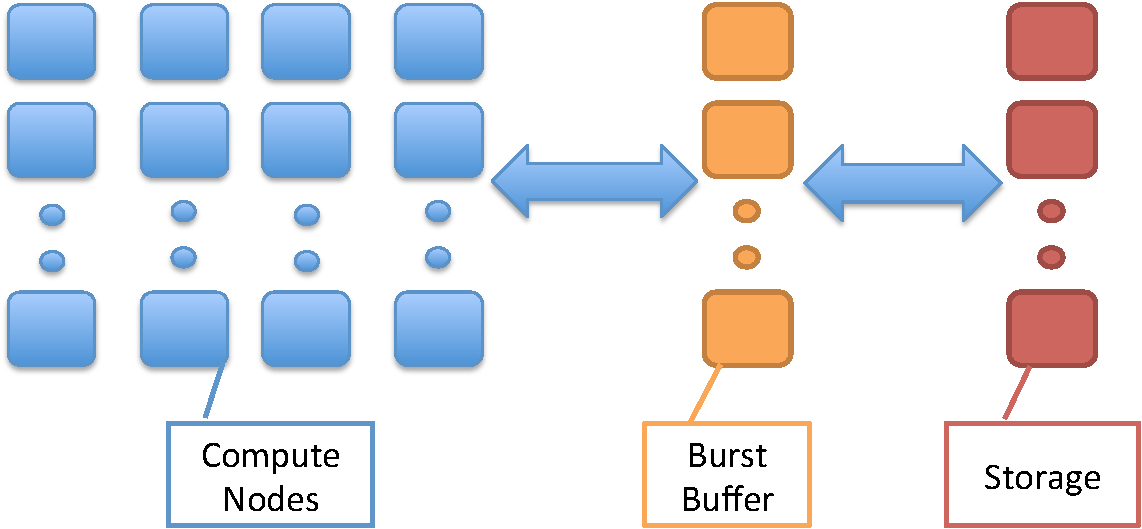
\includegraphics[width=8cm]{img/burst_buffer.pdf}
\caption{burst buffer architecture}
\label{background:burst buffer architecture}
\end{figure}

Modern high performance systems consist of thousands of compute nodes, and hundreds of
applications are running at the same time, some I/O request peak can hardly be meet by current
storage hierarchy. 
Traditional approach, which solves such problem by providing a higher bandwidth storage will cause
the storage system under utilization.
Previous research\cite{on_the_role_of_burst_buffers} proposed a
burst buffer system as a new tier of current storage hierarchy.
Burst buffer system uses several local compute nodes as a burst buffer to absorb I/O
request. 
By adding such new tier of storage hierarchy, temporal I/O request can be absorb by burst buffer
without a need of higher bandwidth storage. Figure~.\ref{background:burst buffer architecture}
shows the architecture of burst buffer.

Such burst buffer system can burst the application which has a high data locality I/O pattern, since
the data can be read once from storage and then buffered in the burst buffer system, subsequent
request for the same data can be accessed from burst buffer.
Furthermore, applications which write a lot also can benefit from burst buffer system, by buffering
output data in burst buffer, application can go ahead without waiting data be finally write to
storage.

\subsection{Data Locality}
\begin{comment}
add other kinds of application data locality details.
as more as possible
\end{comment}

\begin{table}
\centering
\begin{tabular}{|c|p{150pt}|}
\hline
Montage		&		a portable software toolkit for constructing custom, science-grade 
mosaics by composing multiple astronomical images\cite{montage}.\\\hline
pov ray		&		a ray tracing program which generates images from a text-based scene description, and is
available for a variety of computer platforms\cite{povray}.\\\hline
Supernovae	&	a program use SExtractor\cite{SExtractor}, a program that builds a catalogue of objects
from an astronomical image and CFITSIO\cite{fitsio},  a library of C and Fortran subroutines for
reading and writing data files in FITS (Flexible Image Transport System) data format to find supernovae in a set of
astronomical image.\\
\hline
\end{tabular}
\caption{Work Flow Applications}
\label{background:work flow applications}
\end{table}

\begin{figure}
\centering
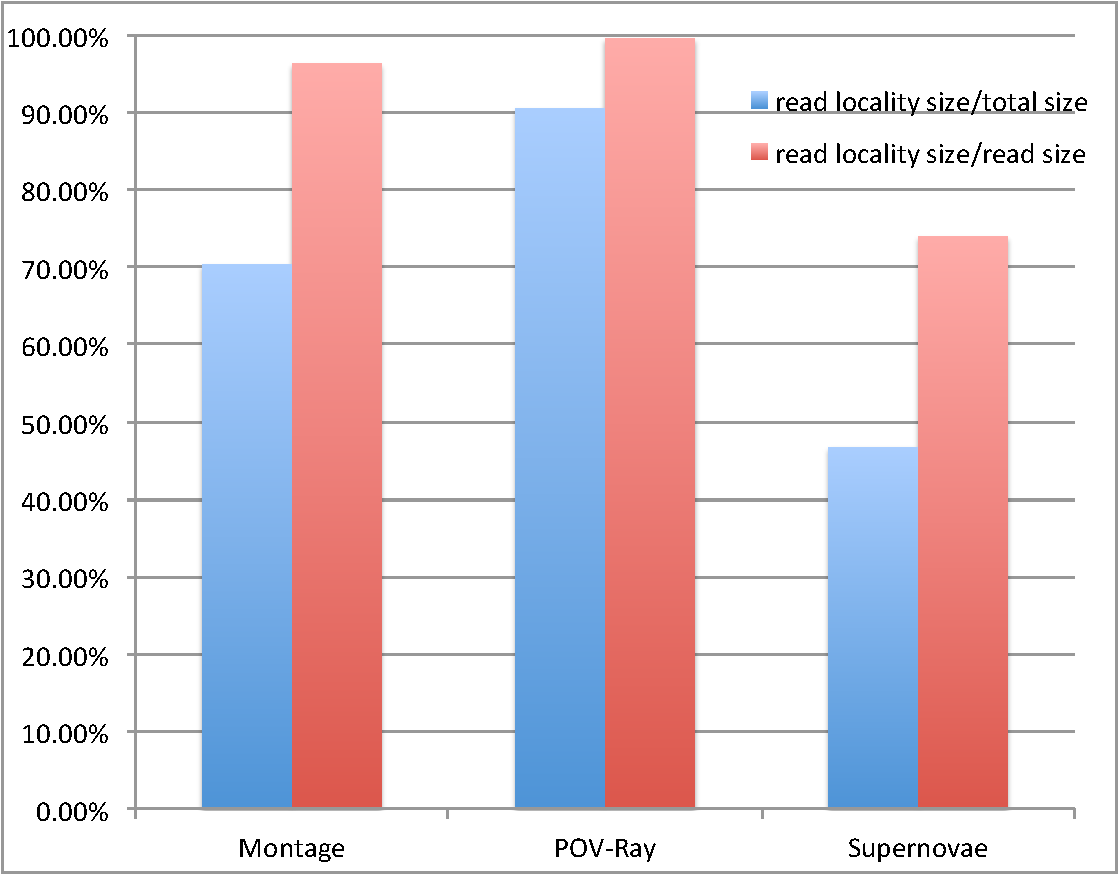
\includegraphics[width=8cm]{img/data_locality.pdf}
\caption{Data Locality}
\label{background:data locality}
\end{figure}
\xtq{what is muse?what can muse do?how to use muse to get data locality}
Data locality is a phenomenon describing the same value, or related storage locations, being
frequently accessed.
Technology like cache, instruction prefetch for memory, or the advanced branch predictor
at the pipelining of processors is based on this phenomenon.
Many previous research investigated data locality of various
applications including 
mapreduce,\cite{Investigation_of_Data_Locality_in_MapReduce}, scientific
\cite{Intrinsic_data_locality_of_modern_scientific_workloads},
OLTP\cite{Data_locality_characterization_of_OLTP},
numeric\cite{Analyzing_data_locality_in_numeric_applications}etc., and showed that these
applications has a strong data locality.
Among these applications, work flow applications shows a strongest data locality, in this paper, we
focus on work flow applications.
Since our proposal
system buffer I/O data and as previous section shows the buffered data can be accessed in a high throughput, applications' I/O data locality will affect the performance gains by
using our propose system greatly, So we measure the I/O data locality for the applications.
\xtqmod{
We use MUSE\cite{MUSE}, which is a tool to monitor file open, close, read, write operations
including read/write address, read/write time, and the sizes,
to measure applications data access locality, result is shown in Table~\ref{background:work
flow applications}.}
We count the duplicated read at the same position and all write as data locality size, since all
these cases data can be read from or write to buffer.
Figure~.\ref{background:data locality} shows the results of these three applications.
We can see
that the I/O pattern of all the three applications shows a strong data locality. Montage and Pov ray
are over 90\% and supernovae achieved over 80\%.
